\newpage
\section{Definitionen \& Formate}
List aller Codex und Datei-Formate die während des Projektes zum Einsatz kamen.

%%%%%%%%%%%%%%%%%%%%%%%%%%%%%%%%%%%%%%%%%%%%%%%%%%%%%%%%%%%%%%%%%%%%%%%%%%%%%%%
\subsection{webm}
..

\begin{verbatim}
<video width="320" height="240" controls>
  <source src="movie.ogg" type="video/webm">
  Your browser does not support the video tag.
</video> 
\end{verbatim}

%%%%%%%%%%%%%%%%%%%%%%%%%%%%%%%%%%%%%%%%%%%%%%%%%%%%%%%%%%%%%%%%%%%%%%%%%%%%%%%
\subsection{ogg}

\textbf{WIKIpedia - rewrite - Zusammenfassen}
Achtung, kann auch direkt auf einer Website dargestellt werden!\\

Ogg ist ein Container-Dateiformat für Multimedia-Dateien, kann also gleichzeitig Audio-, Video- sowie Textdaten enthalten. Ogg wurde mit dem Ziel konzipiert, eine freie und von Softwarepatenten unbeschränkte Alternative zu proprietären Formaten zu bieten, um Multimedia-Inhalte effizient zu speichern und zu streamen. Die Streamingfähigkeit ist dabei das entscheidende Designmerkmal: Alles, was in einem Ogg-Container verpackt ist, kann ohne zusätzliche Anpassungen gestreamt werden. Dies unterscheidet Ogg von Formaten, die entweder nur in bestimmten Ausprägungen streamingfähig sind (wie z. B. Matroska) oder überhaupt nicht live-streaming-fähig sind (wie z. B. MP4). Ogg-Streams können dabei gebündelt und verkettet werden, ohne dass dazu eine Anpassung des einzelnen Streams notwendig ist.[2]

Die Entwicklung des Container-Formats wird von der Xiph.Org Foundation geleitet, die auch für einige Codecs verantwortlich ist, welche die Inhalte in einem Ogg-Container komprimieren.

Der bekannteste Codec ist dabei der Audio-Codec Vorbis, welcher oft vereinfachend (oder auch irrtümlich) als Ogg bezeichnet wird, obwohl Ogg tatsächlich nur das Containerformat für die Vorbis-kodierten Inhalte ist. In jüngerer Vergangenheit (seit 2012) setzt sich auch das Vorbis-Nachfolgeformat Opus langsam durch, insbesondere auch im professionellen Broadcast-Umfeld in Hardware-Audio-Codecs. 


\begin{verbatim}
<video width="320" height="240" controls>
  <source src="movie.ogg" type="video/ogg">
  Your browser does not support the video tag.
</video> 
\end{verbatim}

%%%%%%%%%%%%%%%%%%%%%%%%%%%%%%%%%%%%%%%%%%%%%%%%%%%%%%%%%%%%%%%%%%%%%%%%%%%%%%%
\subsection{mp4}



\begin{verbatim}
<video width="320" height="240" controls>
  <source src="movie.mp4" type="video/mp4">
  Your browser does not support the video tag.
</video> 
\end{verbatim}

%%%%%%%%%%%%%%%%%%%%%%%%%%%%%%%%%%%%%%%%%%%%%%%%%%%%%%%%%%%%%%%%%%%%%%%%%%%%%%%
\subsection{h264}

Beschreibung von h264 Nutzen...

\begin{minipage}{\textwidth}
    \begin{center}
        Caption for image
        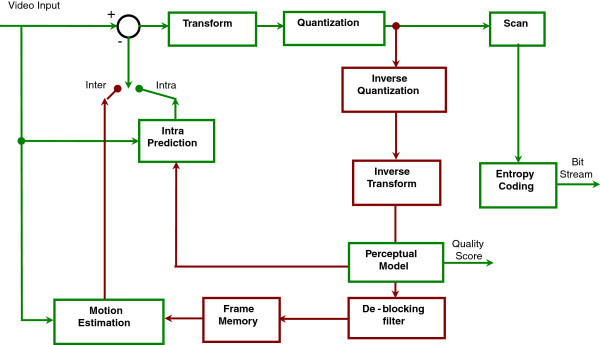
\includegraphics[scale=4.0]{img/h264.jpg} 
    \end{center}
\end{minipage}




%%%%%%%%%%%%%%%%%%%%%%%%%%%%%%%%%%%%%%%%%%%%%%%%%%%%%%%%%%%%%%%%%%%%%%%%%%%%%%%
\newpage
\section{Vergleich der Formate}

\subsection{RTMP versus WebRTC}
RTMP/RTSP are better for livestreaming in ‘live’ meaning. We can easily reduce the latency of RTMP or RTSP to around 1 second with just some simple setup and a good connection to the server, many streaming apps are using RTMP protocol nowaday. The only and biggest weakness of RTMP is it requires Flash and is not easily to be integrated into a website\\

WebRTC is something called the future for livestreaming, it is a peer-to-peer protocol which can reach ‘realtime’ latency for livestreaming(under 1 second). The weakness of WebRTC is it is hard when we need scaling, currently it is just approriate livestreaming in online meeting which require a small value of peers. There are many solution to overcome this, such as a hybrid solution combining WebRTC for input and RTMP/HLS/DASH for output.














%\section*{Format ogg}  no number!



